\documentclass[a4paper]{article}

\usepackage{xltxtra}
\XeTeXlinebreaklocale "th_TH" 
\XeTeXlinebreakpenalty = 100
\XeTeXlinebreakskip = 0pt plus 1pt
\linespread{1.5}
\setmainfont[
    Scale = MatchUppercase,
    Mapping = tex-text
]{TH Sarabun New}
\newfontfamily{\thaifont}[
    Scale = MatchUppercase,
    Mapping = tex-text
]{TH Sarabun New}

\renewcommand{\abstractname}{บทคัดย่อ}
\renewcommand{\figurename}{รูปที่}
\renewcommand{\tablename}{ตารางที่}
\renewcommand{\refname}{บรรณานุกรม}

\usepackage[
    top = 2.54cm,
    bottom = 2.54cm,
    left = 2.54cm,
    right = 2.54cm
]{geometry}

\graphicspath{{./images/}}

\usepackage[numbib]{tocbibind}
\usepackage[justification = centering]{caption}
\usepackage{indentfirst}
\usepackage{pgfplots}
\usepackage{pgfplotstable}
\pgfplotsset{compat = 1.18}

\title{การเปลี่ยนแปลงสัทลักษณะของเสียงวรรณยุกต์จัตวา\\ในภาษาไทยกรุงเทพ}
\author{
    ปานญุตม์ ศรีวิโรจน์\\6340138322
    \and
    อภิมณฑ์ จิตรอักษร\\6340261822
    \and
    วราลี วงษ์สมตระกูล\\6340209222
    \and
    สุชญา สุรพนานนชัย\\6340241222
}
\date{}

\begin{document}
\maketitle
\begin{abstract}
    แม้ว่าจะมีการศึกษาสัทลักษณะของเสียงวรรณยุกต์ไทยค่อนข้างมาก แต่การศึกษาเปรียบเทียบเสียงวรรณยุกต์ภาษาไทยในกลุ่มช่วงอายุของผู้พูดที่แตกต่างกันยังไม่แพร่หลายนัก ทั้งที่เป็นประเด็นที่น่าสนใจศึกษา จากการที่ผู้สูงอายุส่วนมากมักจะมองว่าเสียงวรรณยุกต์ของคนรุ่นใหม่เป็นเสียงที่ค่อนข้าง “แบน” หรือไม่มีการขึ้น-ลงของเสียงวรรณยุกต์มากนัก  และเสียงวรรณยุกต์จัตวาซึ่งเป็นเสียงที่มีลักษณะการขึ้น-ลง (contour) อย่างชัดเจนก็เป็นอีกหนึ่งเสียงที่จะเกิดความแตกต่างในการพูดให้แบนขึ้นหรือมีความชันลดลงตามอายุของผู้พูดได้ การศึกษานี้จึงมุ่งศึกษาความแตกต่างระหว่างเสียงวรรณยุกต์จัตวาของผู้พูดที่มีอายุแตกต่างกัน โดยเก็บข้อมูลจากผู้พูดภาษาไทยกรุงเทพ 15 คนที่มีอายุตั้งแต่ 19 ปีจนถึง 83 ปี เพื่อทดสอบสมมติฐานว่าเมื่อผู้พูดมีอายุลดลง สัทลักษณะด้านความชันโดยรวมทั้งวรรณยุกต์จัตวาจะลดลง และตำแหน่งจุดหักเหของวรรณยุกต์จัตวาจะไกลกว่าผู้พูดที่มีอายุมากกว่าจริงหรือไม่ ผลการศึกษาที่พบสอดคล้องกับสมมติฐานที่ตั้งไว้ทั้ง 2 ข้อ และสามารถสรุปได้ว่าอายุเป็นปัจจัยสังคมที่ส่งผลต่อการแปรสัทลักษณะของวรรณยุกต์จัตวาในภาษาไทยกรุงเทพอย่างมีนัยสำคัญทางสถิติ
\end{abstract}
\section{บทนำ}
    จากงานวิจัยที่ศึกษาเรื่องการเปลี่ยนแปลงของเสียงวรรณยุกต์ในภาษาไทยกรุงเทพหรือภาษาไทยมาตรฐานจะพบว่ามีการเปลี่ยนแปลงสัทลักษณะของแต่ละวรรณยุกต์อยู่ตลอดตั้งแต่อดีตจนถึงปัจจุบัน (Thepboriruk, 2010) อย่างไรก็ตาม วรรณยุกต์จัตวา (Rising Tone) เป็นวรรณยุกต์ที่ไม่มีการเปลี่ยนแปลงมากนักเมื่อเทียบกับวรรณยุกต์อื่น ๆ เช่น วรรณยุกต์โท (High Tone) เพราะนับตั้งแต่การศึกษาสัทลักษณะของเสียงวรรณยุกต์จัตวาโดย Abramson (1962) จนถึงปัจจุบันก็ยังพบว่าวรรณยุกต์จัตวามีลักษณะคล้ายเดิม คือ เป็นเส้นโค้งที่เสียงจะตกลงก่อนขึ้นเสียงสูง

    นอกจากการแปรเสียงวรรณยุกต์จะแตกต่างกันตามช่วงเวลาแล้ว ในผู้พูดที่แตกต่างกันก็พบการใช้เสียงวรรณยุกต์ที่แตกต่างกันเช่นเดียวกัน โดยมีแนวโน้มว่า ความหลากหลายของรูปแปรวรรณยุกต์จะแปรผกผันกับการเคลื่อนไหวในวรรณยุกต์ (Tonal Movement) กล่าวคือ วรรณยุกต์ที่มีการเคลื่อนไหวในวรรณยุกต์มาก อย่างเสียงจัตวาและเสียงโท จะพบการแปรที่น้อยกว่าเสียงวรรณยุกต์ที่มีการเคลื่อนไหวในวรรณยุกต์น้อยกว่า อย่างเสียงสามัญและเสียงเอก (Gandour et al, 1991)

    ปัจจัยทางสังคมอีกประการหนึ่งที่มีผลต่อการแปรของเสียงวรรณยุกต์ค่อนข้างมากคืออายุ ซึ่งเป็นปัจจัยที่มีการศึกษากล่าวถึงค่อนข้างมาก รวมทั้งมีข้อสังเกตที่ว่าผู้พูดภาษาไทยที่มีอายุน้อยมักจะมีการพูดเสียงลอย ๆ กล่าวคือ มีเสียงวรรณยุกต์หลายเสียงที่ไม่ขึ้นหรือตกอย่างชัดเจนแบบเดียวกันทั้งหมด (อรุณี อรุณเรือง, 2533) ซึ่งสอดคล้องกับคำพูดของผู้สูงอายุที่มักจะบอกว่าวรรณยุกต์ของคนรุ่นใหม่ค่อนข้างแบน (Flat) และจากการศึกษากลุ่มผู้พูดภาษาไทยกรุงเทพเปรียบเทียบกันสามช่วงอายุ ก็พบว่าผู้พูดที่มีอายุน้อยมีแนวโน้มที่จะมี ช่วงเสียง (Pitch Range) ที่ต่ำกว่า และจะมีการเปลี่ยนแปลงทางเสียงที่ช้ากว่า (Later Pitch) ในเส้นความโค้ง (Contour) ของเสียงวรรณยุกต์จัตวา (Thepboriruk, 2010)

    ด้วยเหตุนี้ ผู้ศึกษาจึงสนใจศึกษาการแปรสัทลักษณะของวรรณยุกต์จัตวาหรือ Rising Tone ในผู้พูดภาษาไทยกรุงเทพที่มีช่วงอายุแตกต่างกัน เนื่องจากวรรณยุกต์จัตวาเป็นเสียงวรรณยุกต์ที่ดูมีความคงที่ ไม่ได้มีการเปลี่ยนแปลงในภาพรวมตามเวลามากนัก และมีแนวโน้มที่จะมีรูปแปรที่ค่อนข้างน้อย หากมีการเปลี่ยนแปลงที่เกิดขึ้นในปัจจุบันอาจเป็นการเปลี่ยนแปลงที่มีนัยสำคัญบางอย่างได้

    นอกจากนี้แล้ว งานวิจัยที่ศึกษาการแปรสัทลักษณะของเสียงวรรณยุกต์ตามช่วงอายุส่วนมากเป็นงานวิจัยที่ผ่านมาหลายปีแล้ว กลุ่มผู้พูดภาษาไทยที่อายุน้อยอาจเปลี่ยนไปเป็นคนละกลุ่มกับในปัจจุบัน นั่นคือ ผู้พูดภาษาไทยที่อายุน้อยในอดีตจะมีอายุมากขึ้นจนกลายเป็นกลุ่มผู้พูดที่มีอายุอยู่ในช่วงวัยกลางคน ในขณะที่กลุ่มผู้พูดภาษาไทยที่อายุน้อยจะมีกลุ่มใหม่เข้ามาแทนที่ จึงอาจทำให้เกิดการเปลี่ยนแปลงในสัทลักษณะวรรณยุกต์ที่แตกต่างไปจากข้อสังเกตเดิม
\section{ทบทวนวรรณกรรม}
\subsection{ภาษาไทยกรุงเทพ}
    ภาษาไทยกรุงเทพกับภาษาไทยมาตรฐานเป็นสิ่งเดียวกัน เป็นภาษาที่มักจะใช้ในงานราชการ สื่อกระแสหลัก และแสดงถึงเกียรติยศทางสังคมบางอย่าง เห็นได้จากการที่ผู้พูดภาษาไทยที่ไม่ใช่คนกรุงเทพจะพยายามพูดโดยใช้สำเนียงไทยกรุงเทพเมื่อพูดภาษาไทยมาตรฐาน (Tienmee, 1992)

    เสียงวรรณยุกต์ในภาษาไทยกรุงเทพแบ่งออกเป็น 5 เสียงที่แตกต่างกันอย่างชัดเจน ได้แก่ เสียงสามัญ (Mid Tone) เสียงเอก (Low Tone) เสียงโท (Falling Tone) เสียงตรี (High Tone) และเสียงจัตวา (Rising Tone) โดยประเภทของพยางค์ในภาษาไทยจะมีส่วนในการกำหนดเสียงวรรณยุกต์ของคำนั้น ๆ ด้วย ขึ้นอยู่กับว่าพยางค์นั้นเป็นพยางค์เปิดหรือพยางค์ปิด อย่างไรก็ตาม ในช่วงเวลาที่แตกต่างกัน อาจมีความแตกต่างในเส้นโค้งที่แสดงเสียงโท เสียงตรี และเสียงจัตวาอยู่บ้าง

    อย่างไรก็ตาม การศึกษาพบว่าแนวโน้มโดยรวมของผู้พูดภาษาไทยกรุงเทพจะมีการใช้เสียงวรรณยุกต์ที่มีการเปลี่ยนแปลงมากกว่าผู้พูดภาษาไทยที่ไม่ได้อยู่ในกรุงเทพ โดยผู้พูดภาษาไทยที่ไม่ได้อยู่ในกรุงเทพมักจะมีรูปแบบการพูดตามหลักและมีรูปแบบคล้ายกับผู้พูดภาษาไทยกรุงเทพที่มีอายุมากด้วย (Anivan, 1988, as cited in Thepboriruk, 2010)

    ดังนั้น การศึกษานี้จึงมุ่งเน้นศึกษาภาษาไทยกรุงเทพเป็นหลัก เนื่องจากเป็นภาษาไทยที่เป็นมาตรฐานที่สุด และมีแนวโน้มที่จะเกิดการเปลี่ยนแปลงในการใช้เสียงวรรณยุกต์มากกว่า
\subsection{การเปลี่ยนแปลงของวรรณยุกต์ในภาษาไทย}
    ในช่วงต้นศตวรรษที่ 20 งานวิจัยหลายงานเห็นตรงกันว่าเสียงสามัญ (Middle) กับเสียงเอก (Depressed) ในภาษาไทยจะเป็นเสียงที่ค่อนข้างคงที่ (static) แต่เสียงสามัญจะมีการตกลงเล็กน้อยในพยัญชนะท้าย เสียงตรี (Circumflex) จะมีการเพิ่มขึ้นเล็กน้อยและคงที่สักระยะ ก่อนจะตกลงค่อนข้างมากในตอนท้าย ส่วนเสียงจัตวาจะยังไม่มีการโค้งลง แต่จะเป็นเสียงสูงขึ้นไปอย่างเดียว (Bradley, 1909 as cited in Thepboriruk, 2010)
    \begin{figure}[!ht]
        \begin{center}
        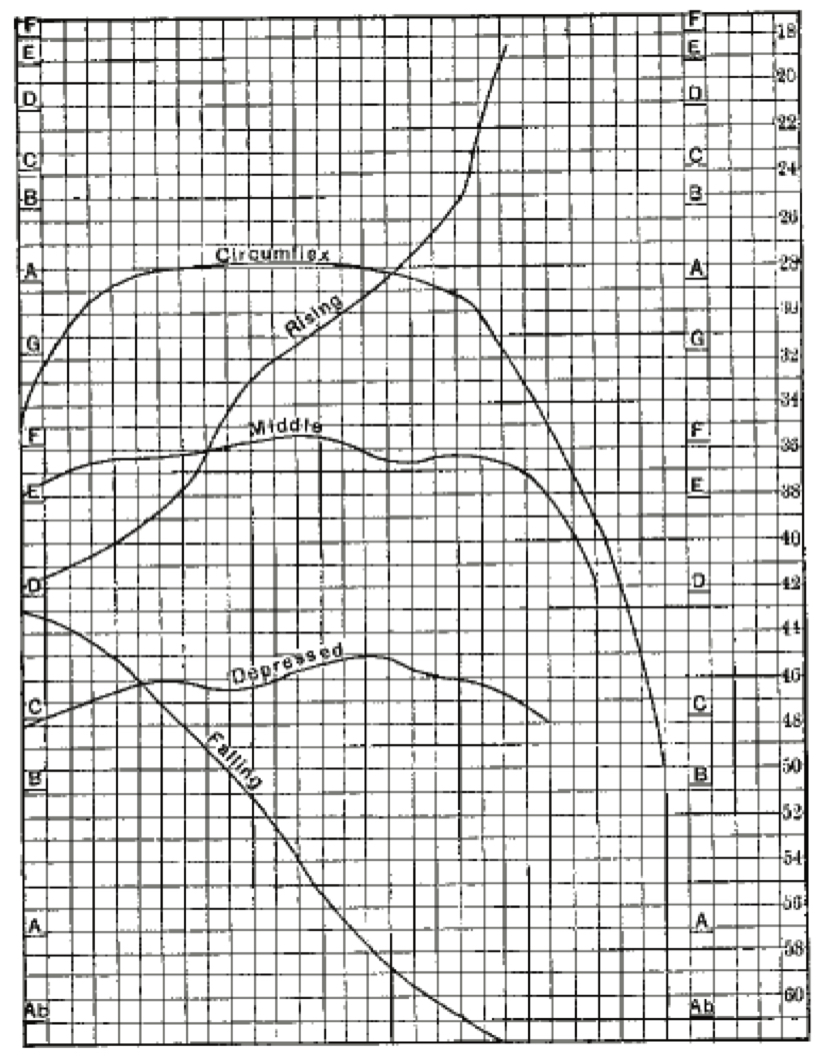
\includegraphics[width=0.5\textwidth]{bradley}
        \end{center}
        \caption{เสียงวรรณยุกต์ภาษาไทยโดย Bradley (1909)}
    \end{figure}

    ต่อมา Abramson (1962 as cited in Thepboriruk, 2010) ถึงเริ่มพบการโค้งของเสียงจัตวา โดยจะเริ่มจากตกก่อนเล็กน้อยแล้วค่อยตามมาด้วยเสียงที่สูงขึ้นอย่างรวดเร็ว ซึ่งแตกต่างจากการศึกษาเก่า เสียงตรีและเสียงสามัญจะค่อนข้างคงที่ แต่มีการตกลงเล็กน้อยในช่วงท้าย ในขณะที่เสียงเอกจะมีการตกลงก่อนเล็กน้อยแล้วจึงค่อยคงที่ในครึ่งหลัง ส่วนเสียงโทจะมีการขึ้นสูงก่อนจะคงที่สักระยะ และตกลงอย่างรวดเร็วและชัดเจน
    \begin{figure}[!ht]
        \begin{center}
        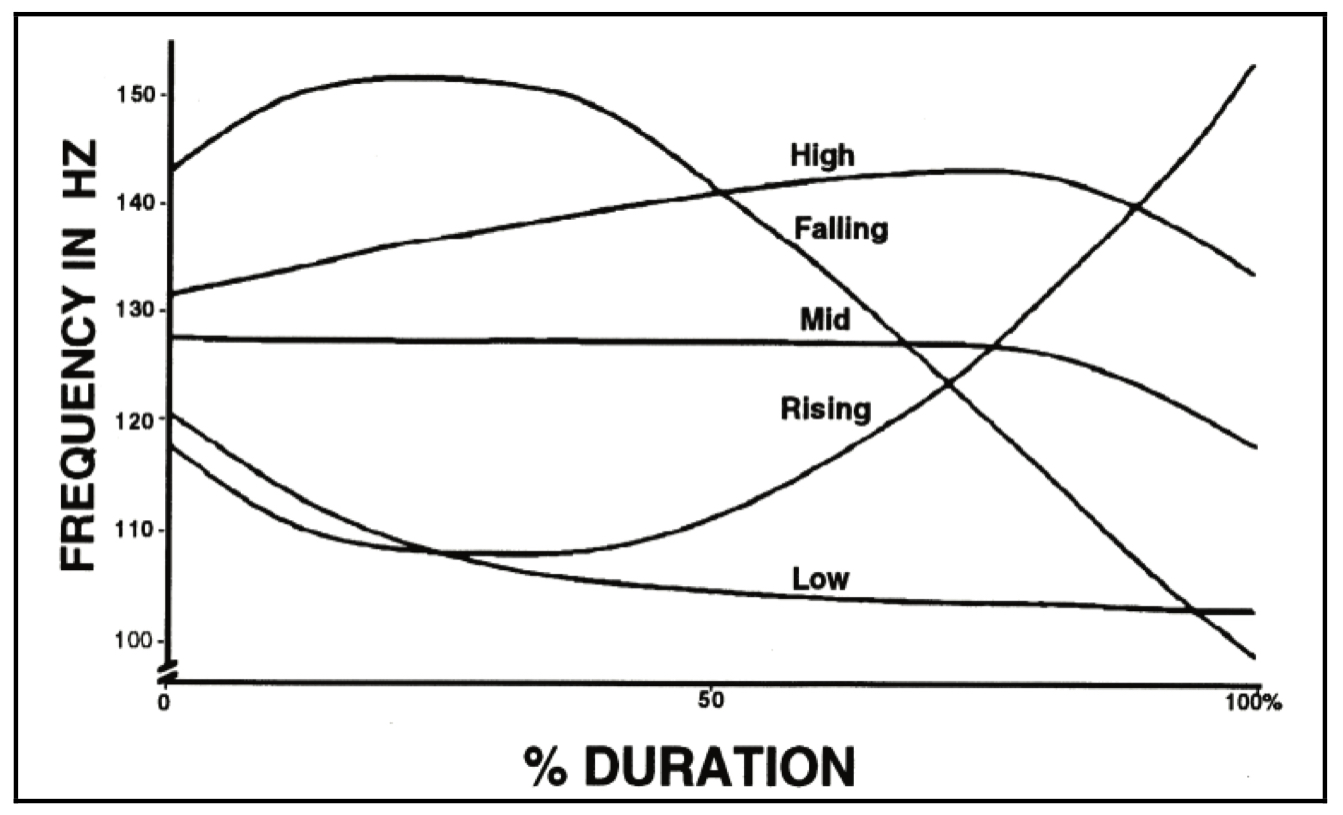
\includegraphics[width=0.5\textwidth]{abramson}
        \end{center}
        \caption{เสียงวรรณยุกต์ภาษาไทยโดย Abramson (1962)}
    \end{figure}

    Ganduar et al (1991, as cited in Thepboriruk, 2010) ที่ศึกษาเสียงวรรณยุกต์ในผู้พูดหลายคนที่มีความแตกต่างก็พบผลการศึกษาที่มีรูปแบบเสียงวรรณยุกต์โดยรวมสอดคล้องกับงานก่อนหน้านี้เช่นกัน และนอกจากนี้ยังพบว่าความหลากหลายของรูปแปรวรรณยุกต์จะแปรผกผันกับการเคลื่อนไหวในวรรณยุกต์ (Tonal Movement) กล่าวคือ วรรณยุกต์ที่มีการเคลื่อนไหวในวรรณยุกต์มาก อย่างเสียงจัตวาและเสียงโท จะพบการแปรที่น้อยกว่าเสียงวรรณยุกต์ที่มีการเคลื่อนไหวในวรรณยุกต์น้อยกว่า อย่างเสียงสามัญและเสียงเอก

    อย่างไรก็ตาม งานของ Morén \& Zsiga (2006, as cited in Thepboriruk, 2010) ในเวลาต่อมา พบรูปแบบเสียงวรรณยุกต์ที่แตกต่างออกไป เนื่องจากเสียงตรีและจัตวาได้เปลี่ยนแปลงจนมีเส้นโค้งที่ค่อนข้างคล้ายกันแล้ว คือเริ่มจากตกเล็กน้อยและคงที่ในระยะหนึ่ง ก่อนจะขึ้นเสียงสูงในช่วงท้าย แต่จะแตกต่างกันในค่า F0 ของจุดเริ่มต้น ส่วนเสียงโทและเสียงเอกจะยังคล้ายเดิม โดยที่เสียงเอกจะมีความเป็นเส้นตรงมากขึ้น เสียงตกลงอย่างคงที่ตั้งแต่จุด onset ถึง offset
    \begin{figure}[!ht]
        \begin{center}
        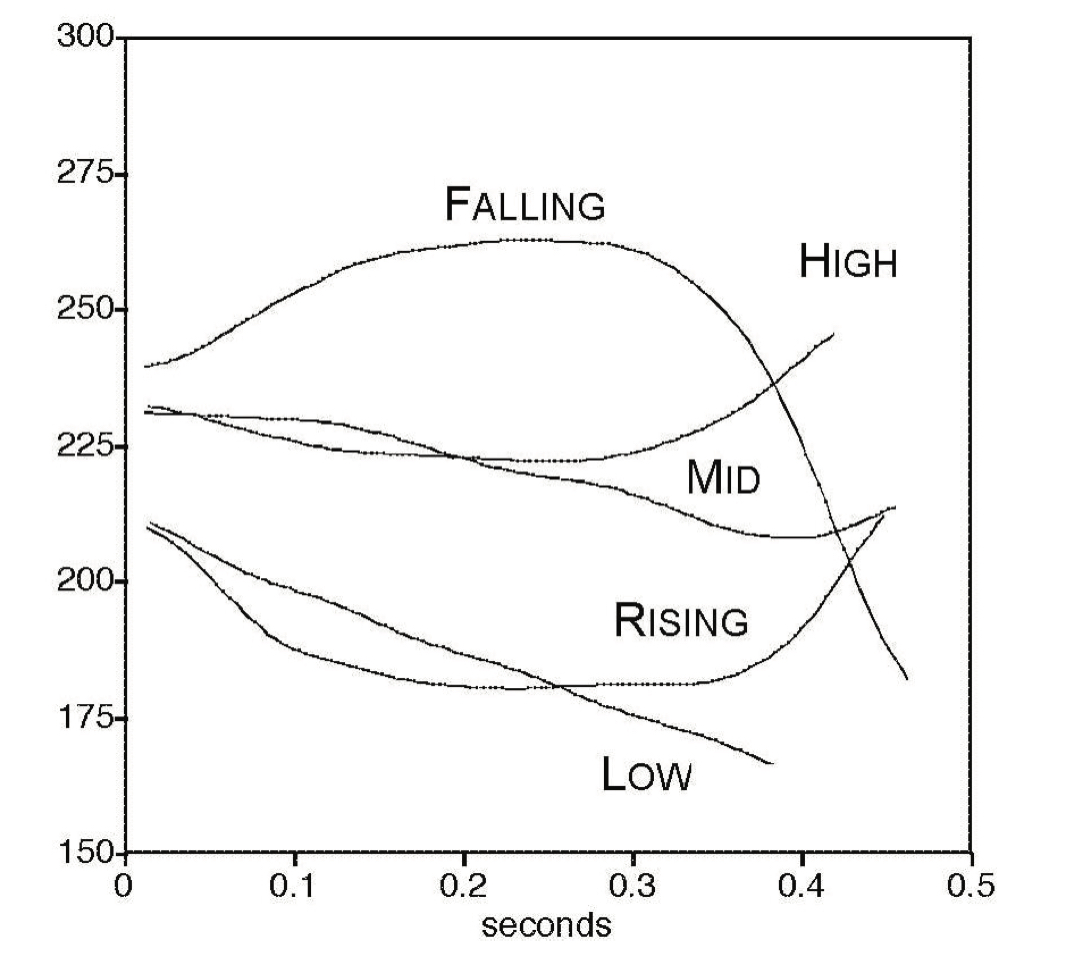
\includegraphics[width=0.5\textwidth]{zsiga}
        \end{center}
        \caption{เสียงวรรณยุกต์ภาษาไทยโดย Morén \& Zsiga (2006)}
    \end{figure}

    จากงานวิจัยตั้งแต่อดีตจนถึงปัจจุบัน จะเห็นได้ว่าเสียงวรรณยุกต์ในภาษาไทยมีการเปลี่ยนแปลงทางสัทลักษณะอยู่เรื่อย ๆ แต่เสียงวรรณยุกต์จัตวาในช่วงแรกจะเป็นเสียงที่ขึ้นเสียงเพียงอย่างเดียว แต่หลังจากนั้นจะมีลักษณะเป็นเส้นโค้งที่ค่อนข้างใกล้เคียงเดิม ไม่ได้มีการเปลี่ยนแปลงในรูปแบบที่ชัดเจนนัก ต่างจากเสียงตรีที่มีการเปลี่ยนแปลงค่อนข้างมากก่อนจะกลายมาเป็นเส้นโค้งที่มีลักษณะคล้ายเสียงจัตวาในปัจจุบัน

    นอกจากนี้ งานส่วนมากเกี่ยวกับการศึกษาเสียงวรรณยุกต์ภาษาไทยจะเน้นศึกษาไปที่การออกเสียงเป็นคำ ๆ ตามรูป (Citation-form pronunciation) มากกว่าจะศึกษาคำที่พูดต่อเนื่องกันยาว ๆ ทั้งนี้ Noss (1975, as cited in Thepboriruk, 2010) ได้ให้เหตุผลไว้ว่าการออกเสียงคำตามรูปแบบนี้เป็นพื้นฐานของการทำความเข้าใจเสียงวรรณยุกต์ไทย และจำเป็นต่อการศึกษาทั้งด้านสัทศาสตร์และสัทวิทยา ดังนั้น ผู้ศึกษาจึงเลือกที่จะศึกษาเสียงวรรณยุกต์จัตวาจากข้อมูลการออกเสียงตามรูปเป็นคำ ๆ เพื่อเป็นพื้นฐานกับงานวิจัยอื่น ๆ และเพื่อให้เห็นการเปรียบเทียบที่ชัดเจนกับงานวิจัยเก่า ๆ ด้วย
\subsection{การแปรสัทลักษณะของวรรณยุกต์ตามช่วงอายุของผู้พูด}
    งานที่ศึกษาวรรณยุกต์ภาษาไทยส่วนมากมักจะไม่ได้แยกความแตกต่างระหว่างกลุ่มอายุของผู้พูด และมองว่าวรรณยุกต์เป็นสิ่งที่คงที่ไม่ว่าจะเป็นเวลาไหนหรือผู้พูดคนใดก็ตาม อย่างไรก็ตาม การศึกษาของ Gandour et al (1991, as cited in Thepboriruk, 2010) ซึ่งเป็นงานชิ้นแรก ๆ ที่ศึกษาผู้พูดภาษาไทยที่มีความหลากหลาย ต่างเพศ และต่างอายุ พบว่าความแตกต่างในการผลิตเสียงวรรณยุกต์ระหว่างกลุ่มผู้พูดที่มีอายุน้อยกับอายุมากมีค่อนข้างน้อย แต่ความแตกต่างที่เกิดจากระดับการศึกษาและสถานะทางเศรษฐกิจและสังคมในกลุ่มผู้พูดที่มีอายุมากกลับมีรูปแบบที่คล้ายคลึงกับในผู้พูดที่มีอายุน้อย

    อย่างไรก็ตาม Thepboriruk (2010) ได้เริ่มศึกษาเปรียบเทียบการใช้เสียงวรรณยุกต์ในกลุ่มผู้พูดภาษาไทยกรุงเทพสามช่วงอายุ ซึ่งนับเป็นการศึกษาปัจจัยทางด้านสังคมเปรียบเทียบระหว่างทั้งห้าวรรณยุกต์ในภาษาไทยกรุงเทพงานแรก ๆ และพบว่าอายุเป็นปัจจัยที่ทำให้เกิดการแปรเสียงวรรณยุกต์จริง โดยผู้พูดที่มีอายุน้อยมีแนวโน้มที่จะพูดเสียงวรรณยุกต์สามัญและเอกสูงกว่า และจะมีการเปลี่ยนแปลงทางเสียงหรือจุดหักเหที่ช้ากว่าในเสียงวรรณยุกต์โทและจัตวาซึ่งเป้นเสียงโค้ง

    งานวิจัยนี้พบการเปลี่ยนแปลงทั้งทางด้านลักษณะ จุด onset และ offset ในเสียงวรรณยุกต์ของผู้พูดในช่วงอายุที่แตกต่างกัน โดยพบว่าวรรณยุกต์ตรีเป็นเสียงที่มีความแตกต่างกันระหว่างกลุ่มผู้พูดแต่ละช่วงอายุมากที่สุด ส่วนเสียงจัตวาจะเป็นเส้นโค้งเหมือนกันทั้งหมดในทุกกลุ่มช่วงอายุ และมีจุด onset ที่ใกล้เคียงกันคือประมาณ 40\% ของเสียง แต่ผู้พูดที่มีอายุน้อยจะมีจุดหักเหของเสียงที่ต่ำมากที่สุดถึงประมาณ 30\% นอกจากนี้ ผู้พูดที่มีช่วงอายุมากและช่วงวัยกลางคนจะมีจุดที่ต่ำที่สุดอยู่ในช่วงประมาณ 50\% ของความยาวของเสียง ในขณะที่ผู้พูดที่มีอายุน้อยจะมีจุดที่ต่ำที่สุดอยู่ในช่วง 60\% แสดงให้เห็นถึงการมีจุดต่ำสุดที่ช้ากว่า (later pitch) อยู่ประมาณ 10\% ของความยาวทั้งหมด นอกจากนี้ ผู้พูดที่มีอายุน้อยจะมีระดับเสียงโดยรวมที่ต่ำกว่ากลุ่มผู้พูดที่มีอายุมากกว่าด้วย
    \begin{figure}[!ht]
        \begin{center}
        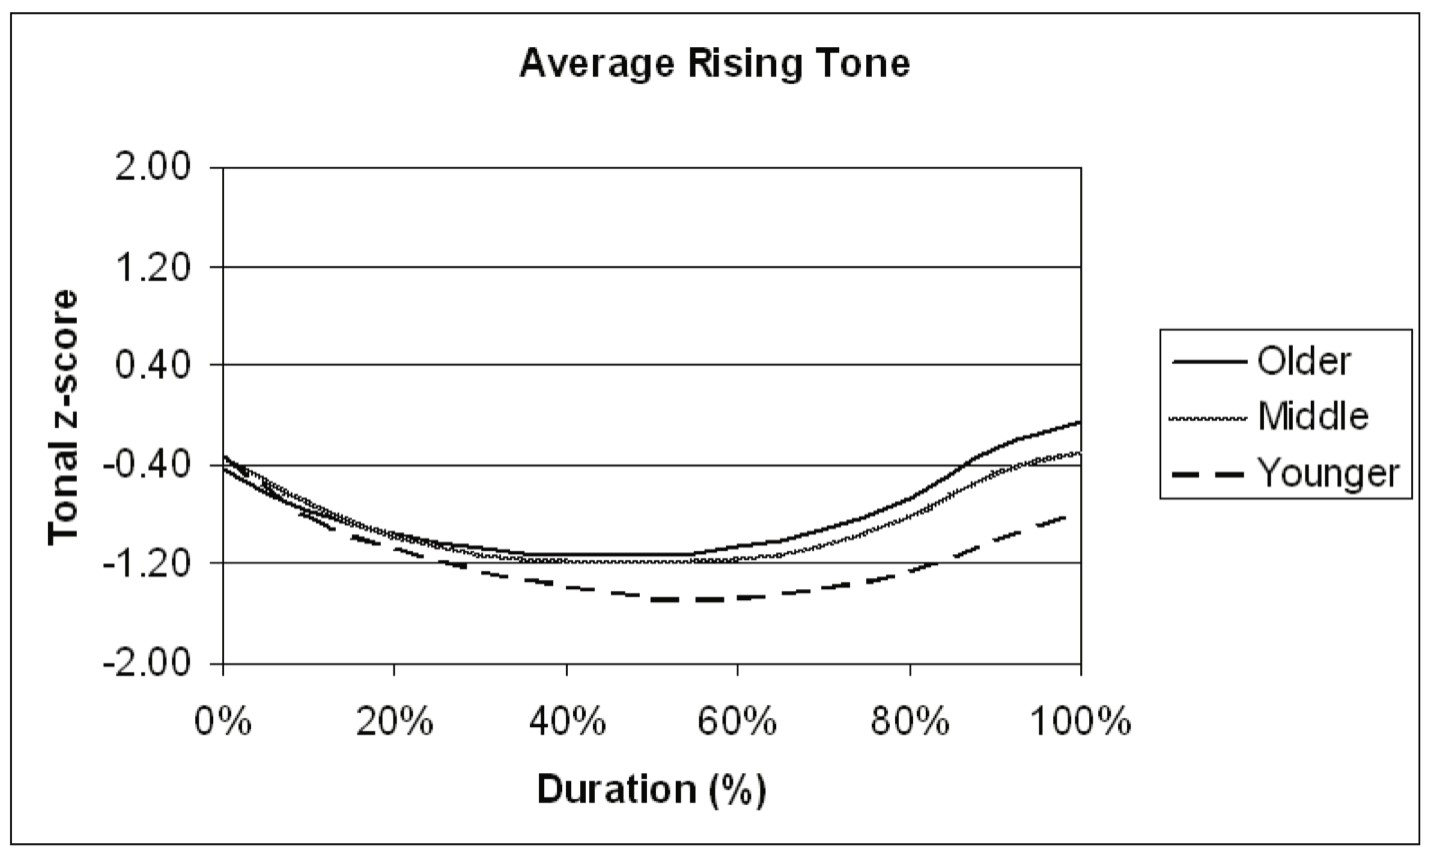
\includegraphics[width=0.5\textwidth]{thepboriruk}
        \end{center}
        \caption{เสียงวรรณยุกต์จัตวาในกลุ่มผู้พูดที่มีช่วงอายุแตกต่างกัน โดย Thepboriruk (2010)}
    \end{figure}
\subsection{การรับรู้วรรณยุกต์ในภาษาไทย}
    ความแตกต่างในด้านการรับรู้ทางสัทศาสตร์อาจส่งผลต่อการรับรู้เสียงวรรณยุกต์ได้ โดย Teeranon (2007, as cited in Thepboriruk, 2010) พบว่าผู้ที่มีอายุต่ำกว่า 20 ปีจะรับรู้เสียงที่มีการโค้งขึ้น-ลงอย่างมากเป็นเสียงตรี ในขณะที่กลุ่มที่มีอายุมากกว่า 60 ปีจะมองว่าเสียงตรีคือเสียงสูงที่มีลักษณะคงที่ และมักจะสับสนเสียงวรรณยุกต์จัตวากับเสียงตรีมากกว่ากลุ่มผู้ที่มีอายุต่ำกว่า 20 ปีอย่างมาก

    ผลการศึกษานี้สอดคล้องกับงานที่ศึกษาเรื่องการรับรู้เสียงวรรณยุกต์ในภาษาไทย (Zsiga, 2008) ที่พบความสับสนระหว่างเสียงวรรณยุกต์จัตวากับวรรณยุกต์ตรีอย่างมากเช่นเดียวกัน โดยพบว่าเสียงวรรณยุกต์จัตวาเป็นเสียงที่รับรู้ได้ยากและเกิดความสับสนมากที่สุด เนื่องจากมีจุดเริ่มต้นที่ใกล้เคียงกับเสียงเอก และหากออกเสียงขึ้นในตอนหลังไม่ชัดก็อาจจะดูเหมือนเสียงเอกที่ไม่มีการโค้งขึ้นของเสียงในช่วงท้าย แต่หากมีการออกเสียงขึ้นเพียงอย่างเดียวหรือออกเสียงในระดับเสียงที่สูงเกินไปก็จะสับสนกับเสียงวรรณยุกต์โทที่มีเส้นโค้งในลักษณะที่คล้ายคลึงกันได้

    นอกจากนี้ จุดหักเหของเสียงยังเป็นอีกหนึ่งปัจจัยสำคัญที่ส่งผลต่อการรับรู้เสียงวรรณยุกต์ด้วย เนื่องจากหากตำแหน่งของจุดหักเหเปลี่ยนไป ผู้ฟังอาจรับรู้เป็นเสียงวรรณยุกต์ที่ต่างออกไปได้ แม้ว่าลักษณะของวรรณยกต์โดยรวมและโค้งขึ้น-ลงจะยังเหมือนเดิมก็ตาม โดยคนส่วนมากจะรับรู้เสียงวรรณยุกต์จัตวาจากการที่จุดหักเหของเสียงอยู่ระหว่างกลางของความยาวเสียงทั้งหมด (Zsiga \& Nitisaroj, 2007, as cited in Thepboriruk, 2010)

    จะเห็นได้ว่าผู้พูดที่มีอายุแตกต่างกันจะมีการรับรู้เสียงวรรณยุกต์ที่แตกต่างกันได้ ซึ่งการรับรู้เสียงวรรณยุกต์นี้ก็อาจส่งผลต่อการออกเสียงวรรณยุกต์ที่แตกต่างกันออกไปของคนในแต่ละช่วงอายุ การศึกษานี้จึงมุ่งเน้นศึกษาการออกเสียงของวรรณยุกต์จัตวาซึ่งเป็นวรรณยุกต์ที่เกิดความสับสนในการรับรู้มากที่สุด โดยมีจุดหักเหของเสียงซึ่งเป็นปัจจัยสำคัญในการรับรู้เสียงวรรณยุกต์เป็นหนึ่งในสัทลักษณะที่ศึกษา
\section{ระเบียบวิธีวิจัย}
    เป้าหมายของการศึกษาครั้งนี้ คือการทดสอบสมมติฐานทั้งสองข้อ ดังนี้ 1) ความชันโดยรวมทั้งวรรณยุกต์จัตวาจะลดลงเรื่อย ๆ เมื่อผู้พูดมีอายุลดลง กล่าวคือ เมื่อผู้พูดมีอายุน้อย ระดับเสียงของจุด onset และ offset ของเสียงวรรณยุกต์จัตวาจะเคลื่อนเข้าใกล้กันมากขึ้นเมื่อเทียบกับผู้พูดที่มีอายุมากกว่า ส่งผลให้ความชันโดยรวมลดลง และ 2)  ตำแหน่งจุดหักเหของวรรณยุกต์จัตวาจะเกิดช้าขึ้น เมื่อผู้พูดมีอายุลดลง กล่าวคือ เมื่อผู้พูดมีอายุน้อยจุดหักเหของเสียงวรรณยุกต์จะเคลื่อนตัวห่างออกไป ทำให้เข้าใกล้จุด offset มากขึ้น ซึ่งสมมติฐานทั้งสองข้อนี้ ผู้ศึกษามองว่าเป็นสาเหตุที่ทำให้เกิดปรากฏการณ์การออกเสียงวรรณยุกต์จัตวาที่ต่างกันออกไปในแต่ละช่วงวัย ทำให้ผู้พูดที่อายุน้อยกว่าถูกมองว่าออกเสียงวรรณยุกต์จัตวาได้ไม่ชัดเจนเท่าผู้พูดที่มีอายุมากกว่า
\subsection{กลุ่มตัวอย่าง}
    ในการศึกษาเรื่องการแปรของวรรณยุกต์จัตวาในภาษาไทยกรุงเทพนี้ ผู้ศึกษาได้ดำเนินการเก็บข้อมูลจากผู้บอกภาษาซึ่งเป็นผู้พูดภาษาไทยกรุงเทพ ทั้งหมด 15 คน ซึ่งมีอายุตั้งแต่ 19 ถึง 83 ปี โดยเลือกผู้บอกภาษาที่มีอายุกระจายกัน เพื่อให้ได้ผลการวิจัยที่ครอบคลุมทุกช่วงอายุ
\subsection{การเก็บข้อมูล}
    ในขั้นตอนดำเนินการเก็บข้อมูล จะทำการสัมภาษณ์ผู้บอกภาษาก่อนเป็นเวลา 15 นาที โดยจะถามประวัติส่วนตัวของผู้บอกภาษา และเลือกคำถามตามหัวข้อที่ผู้บอกภาษาสนใจและสบายใจที่จะพูดคุย จากนั้นจะให้ผู้บอกภาษาอ่านคำตามลิสต์คำศัพท์ที่ประกอบด้วยคำเสียงวรรณยุกต์จัตวาทั้งหมด 26 คำ และคำที่ไม่ใช่เสียงจัตวาซึ่งเป็นคำหลอก โดยผู้บอกภาษาแต่ละคนจะได้รับเซ็ตคำศัพท์ที่มีการสลับลำดับของคำที่แตกต่างกัน และจะอ่านซ้ำทั้งเซ็ต 2 ครั้ง โดยในขั้นตอนทั้งหมดจะเก็บข้อมูลโดยใช้เครื่องอัดเสียง
\subsection{การประมวลผลข้อมูล}
    เมื่อบันทึกเสียงผู้สัมภาษณ์มาแล้วจะนำไฟล์เสียงที่ได้ทั้งหมดมาตัดให้เหลือเพียงส่วนที่เป็นคำจัตวา เพื่อวิเคราะห์การแปรของสัทลักษณะตามตัวแปรอายุ เมื่อคัดเหลือเฉพาะไฟล์เสียงจัตวาแล้ว ทำการปรับตรง (align) ไฟล์เสียงด้วย Montreal Forced Aligner และจะได้ไฟล์ TextGrid มา หลังจากนั้นจะตรวจสอบและแก้ไขไฟล์ TextGrid ที่ได้ด้วยมือ ในกรณีที่ตัวสัทอักษรไม่ตรงกับเสียง ก่อนจะนำข้อมูลไปวิเคราะต่อไป
\subsection{การวิเคราะห์ข้อมูล}
    ในการวิเคราะห์ข้อมูลจะใช้ Praat script วัดค่า F0 ทุก ๆ 10 มิลลิวินาทีของคำ และแปลงค่า F0 ที่ได้เป็น semitone  โดยใช้สูตร $12 \times log_2(\frac{F0}{min\ F0})$ เมื่อ min F0 คือค่า F0 ที่ต่ำที่สุดของผู้พูดแต่ละคน จากนั้นเราจะวัดค่าความชัน ตำแหน่งจุดหักเห ระดับ onset และระดับ offset ของแต่ละคำ โดยมีนิยามดังนี้
    \begin{enumerate}
        \item ความชัน คือ ความแตกต่างระหว่างค่า semitone ณ onset และ offset หารด้วยเวลาที่ใช้ในการออกเสียงวรรณยุกต์ทั้งหมด
        \item ตำแหน่งจุดหักเห คือ ร้อยละของเวลาตั้งแต่ onset จนถึงจุดต่ำสุดของวรรณยุกต์ เมื่อเทียบกับเวลาทั้งหมด
    \end{enumerate}

    เมื่อวัดค่าทั้งสองเรียบร้อยแล้ว เราจะนำค่าที่ได้ไปวิเคราะห์โดยใช้ linear regression model เพื่อหาความสัมพันธ์ระหว่างอายุของผู้บอกภาษากับตัวแปรต่าง ๆ ข้างต้น
\section{ผลการศึกษา}
    จากการทำแบบจําลองการถดถอยเชิงเส้น (linear regression model) ของความชันเทียบกับอายุ พบว่ายิ่งผู้พูดมีอายุมากขึ้น ความชันของวรรณยุกต์จัตวาก็จะมากขึ้นเช่นกัน โดยทุก ๆ 1 ปีที่เพิ่มขึ้น วรรณยุกต์จัตวาจะมีความชันเพิ่มขึ้นประมาณ 0.070547 เซมิโทน/มิลลิวินาที (Multiple $R^2$: 0.09137, Adjusted $R^2$: 0.09024)
    \begin{table}[!ht]
        \begin{center}
        \begin{tabular}{|c|c|c|}
            \hline
            ตัวแปร & ค่าสัมประสิทธิ์ & ระดับนัยสำคัญ \\
            \hline
            อายุ & 0.070547 & p<0.001 \\
            \hline
        \end{tabular}
        \end{center}
        \caption{ผลการศึกษาความชันของวรรณยุกต์จัตวา}
    \end{table}
    \begin{figure}[!ht]
        \begin{center}
        \begin{tikzpicture}
        \begin{axis}[
            xlabel = {อายุ (ปี)},
            ylabel = {ความชัน (เซมิโทน/มิลลิวินาที)},
            clip mode = individual
        ]
            \addplot[only marks, fill opacity = 0] table[
                x = age,
                y = slope
            ]{plot.dat};
            \addplot[ultra thick, orange] table[
                x = age,
                y = {create col/linear regression={y=slope}}
            ]{plot.dat};
        \end{axis}
        \end{tikzpicture}
        \end{center}
        \caption{ผลการศึกษาความชันของวรรณยุกต์จัตวา}
    \end{figure}

    ในลักษณะเดียวกัน เมื่อทำแบบจําลองการถดถอยเชิงเส้นของตำแหน่งจุดหักเหเทียบกับอายุ พบว่ายิ่งผู้พูดมีอายุมากขึ้น ตำแหน่งจุดหักเหของวรรณยุกต์จัตวาจะเข้าใกล้ onset มากขึ้นเรื่อย ๆ โดยทุก ๆ 1 ปีที่เพิ่มขึ้น วรรณยุกต์จัตวาจะมีตำแหน่งจุดหักเหเข้าใกล้ onset มากขึ้นประมาณ 0.19669\% (Multiple $R^2$: 0.08207, Adjusted $R^2$: 0.08093)
    \begin{table}[!ht]
        \begin{center}
        \begin{tabular}{|c|c|c|}
            \hline
            ตัวแปร & ค่าสัมประสิทธิ์ & ระดับนัยสำคัญ \\
            \hline
            อายุ & -0.19669 & p<0.001 \\
            \hline
        \end{tabular}
        \end{center}
        \caption{ผลการศึกษาตำแหน่งจุดหักเหของวรรณยุกต์จัตวา}
    \end{table}
    \begin{figure}[!ht]
        \begin{center}
        \begin{tikzpicture}
        \begin{axis}[
            xlabel = {อายุ (ปี)},
            ylabel = {ตำแหน่งจุดหักเห (\%)},
            clip mode = individual
        ]
            \addplot[only marks, fill opacity = 0] table[
                x = age,
                y = inflection
            ]{plot.dat};
            \addplot[ultra thick, orange] table[
                x = age,
                y = {create col/linear regression={y=inflection}}
            ]{plot.dat};
        \end{axis}
        \end{tikzpicture}
        \end{center}
        \caption{ผลการศึกษาตำแหน่งจุดหักเหของวรรณยุกต์จัตวา}
    \end{figure}
\section{อภิปรายผล}
    จากผล Linear Regression modeling ทำให้สามารถปฏิเสธสมมติฐานว่างได้ ซึ่งแปลว่าอายุมีความสัมพันธ์กับความชันและตำแหน่งจุดหักเหของวรรณยุกต์จัตวาอย่างมีนัยสำคัญทางสถิติ และแสดงให้เห็นว่าผู้พูดที่มีรุ่นอายุต่างกันออกเสียงวรรณยุกต์จัตวาแตกต่างกัน โดยสัทลักษณะด้านความชันโดยรวมทั้งวรรณยุกต์จัตวาจะลดลงเรื่อย ๆ เมื่อผู้พูดมีอายุลดลง และตำแหน่งจุดหักเหของวรรณยุกต์จัตวาจะเกิดช้าขึ้นเมื่อผู้พูดมีอายุลดลง

    ผลการศึกษานี้สอดคล้องกับ Thepboriruk (2010) ที่พบว่า กลุ่มผู้พูดภาษาไทยกรุงเทพที่มีอายุน้อย จะมี Pitch range ของวรรณยุกต์จัตวา (rising) ที่ต่ำที่สุด มีจุดสิ้นสุดของวรรณยุกต์ต่ำกว่ากลุ่มที่มีอายุมากกว่า และจะมีจุดหักเห (rising pitch) ที่ช้ากว่ากลุ่มผู้พูดกลุ่มอื่นประมาณ 10\% ของความยาวทั้งหมด และสนับสนุนข้อเสนอของ Pittayaporn (2007) ที่ว่าผู้พูดที่มีอายุน้อยจะมีการลดความชัน (contour reduction) และมีจุดสูงสุดที่ไกลกว่า (peak sliding) เหมือนที่ผู้สูงอายุชอบกล่าวว่าวรรณยุกต์ของคนรุ่นใหม่ค่อนข้าง "แบน (flat)" ทั้งนี้อาจเป็นเพราะการรับรู้เสียงวรรณยุกต์ที่แตกต่างกันในคนแต่ละช่วงวัยด้วย เนื่องจากวรรณยุกต์จัตวาเป็นวรรณยุกต์ที่รับรู้ได้ยากและสับสนมากที่สุด (Zsiga \& Nitisaroj, 2007) และจากการวิเคราะห์ปัจจัยอื่น คือ เพศ พบว่าไม่มีความสัมพันธ์อย่างมีนัยสำคัญกับความชันและตำแหน่งจุดหักเห

    อย่างไรก็ตามในการศึกษาครั้งนี้มีข้อจำกัดที่ควรพิจารณาประกอบด้วย คือ กลุ่มอายุของข้อมูลที่ใช้ค่อนข้างมีการกระจุกตัวอยู่ในกลุ่ม 18-30 ปี เนื่องจากผู้ดำเนินการเก็บข้อมูลทางภาษาเป็นนิสิตในชั้นปริญญาตรีจึงเลือกสัมภาษณ์ผู้บอกภาษาจำนวนมากที่เป็นเพื่อนนิสิตด้วยกันเพื่อความสะดวกในการเก็บข้อมูล

    นอกจากนี้แล้ว จากการสืบค้นพบว่าการศึกษาเกี่ยวกับวรรณยุกต์จัตวาที่มีอยู่ในฐานข้อมูลงานวิจัยนั้นอยู่ในปริมาณที่ค่อนข้างน้อย จึงมีข้อเสนอแนะให้ผู้ที่สนใจศึกษาเกี่ยวกับประเด็นที่เกี่ยวข้องใช้ผลการศึกษาการแปรสัทลักษณะของวรรณยุกต์จัตวาในภาษาไทยกรุงเทพนี้ในการศึกษาการแปรของเสียงวรรณยุกต์อื่น ๆ หรือศึกษาการแปรสัทลักษณะทางวรรณยุกต์จัตวาในภาษาไทยกรุงเทพกับปัจจัยทางสังคมอื่น ๆ ที่อาจจะเกี่ยวข้องเพิ่มเติม เช่น ระดับการศึกษา หรืออาชีพ
\section{สรุป}
    ผลการศึกษาสอดคล้องกับสมมติฐานที่ตั้งไว้ทั้ง 2 ข้อ นั่นคือ เมื่อผู้พูดภาษาไทยกรุงเทพมีอายุลดลง สัทลักษณะด้านความชันโดยรวมทั้งวรรณยุกต์จัตวาจะลดลง และตำแหน่งจุดหักเหของวรรณยุกต์จัตวาจะไกลกว่าผู้พูดที่มีอายุมากกว่า จึงสามารถตอบคำถามวิจัยได้ว่า อายุเป็นปัจจัยสังคมในการแปรสัทลักษณะของวรรณยุกต์จัตวาในภาษาไทยกรุงเทพจริง
\begin{thebibliography}{9}
    \bibitem{arunee} อรุณี อรุณเรือง. (2533). \textit{การแปรของวรรณยุกต์ไทยกรุงเทพฯ ตามระดับอายุผู้พูด.} (วิทยานิพนธ์ปริญญาอักษรศาสตรมหาบัณฑิต, จุฬาลงกรณ์มหาวิทยาลัย).
    \bibitem{abramson} Abramson, A. S. (1962). The vowels and tones of Standard Thai: Acoustical measurements and experiments. \textit{International Journal of American Linguistics, 28}(2): 1-146.
    \bibitem{gandour} Gandour, Jack, Siripong P, \& Sumalee D. (1991). Inter- and intraspeaker variability in fundamental frequency of Thai tones. \textit{Speech Communication, 10}: 355-372.
    \bibitem{pittayaporn} Pittayaporn, P. (2007). Directionality of tone change, \textit{Proceedings of the 16th International Congress of Phonetic Sciences (ICPhS2007)} (pp. 1421-1424). Dudweiler: Pirrot.
    \bibitem{thepboriruk} Thepboriruk, K. (2010). Bangkok Thai tones revisited. \textit{Journal of the Southeast Asian Linguistics Society, 3}(1), 86-105. Retrieved from https://openresearch-repository.anu.edu.au/handle/1885/8943
    \bibitem{tienmee} Tienmee, W. (1992). Classification by tone shapes and patterns of tonal splits and coalescences [Thai dialects of Thailand]. \textit{The Mon-Khmer Studies Journal, 21}, 229-236. Retrieved from http://sealang.net/sala/archives/pdf8/wanna1992classification.pdf
    \bibitem{yang} Yang, W. \& Yang, C. (2018). Reduction in Dali Nisu tone change-in-progress. In \textit{6th International Symposium on Tonal Aspects of Languages: June. 18-20, 2018} (pp. 46-50). doi:10.21437/TAL.2018-10.
    \bibitem{zsiga} Zsiga, E. C. (2008). Modeling diachronic change in the Thai tonal space. \textit{University of Pennsylvania Working Papers in Linguistics, 13}(1), Article 30. Retrieved from https://repository.upenn.edu/pwpl/vol14/iss1/30
\end{thebibliography}
\end{document}